\chapter{NG-HDMI-TS}
\label{chap:network-transmission}

% \section{仮説}
映像のIP伝送については既に多くの先行研究があり、映像を拠点間などで伝送するための製品なども存在している。

しかし、本論文では、拠点間のIP伝送だけにとどまらず、拠点内の設備までもをIP伝送することをテーマとしている。
拠点内の設備として、カメラやスイッチャー、ディスプレイなどの拠点内の設備までもをIP伝送で行う、Video over IP化にするというテーマである。

そのため、実際に制作の現場にIP伝送を普及させた際に、現在の伝送方法の課題が解決でき、IP伝送を利用することができるのかについて検証する。

% \subsection{Ethernetを活用するメリット}

\ref{chap:introduction}章で、述べた通り、ネットワークを活用することによって活かせるメリットは以下の3つである。

\begin{itemize}
  \item 1本のケーブルで複数や双方向の映像が可能
  \item 伝送スピードの向上
  \item コストダウン
\end{itemize}

しかし、Ethernetを利用するためにはデメリットがある

輻輳
導入コストの

また、映像伝送における重要なポイントは以下の3つである。

\begin{itemize}
  \item 画質、音質の劣化がない
  \item 伝送遅延を一定以下にする必要がある
  \item 安定性がある
\end{itemize}

また、IP伝送のメリットは以下の点である。

\begin{itemize}
  \item ユニキャスト、ブロードキャストが行える
\end{itemize}

これらの点において評価を行う。

% 1
\section{映像制作現場で求められるIP伝送装置の要件}
% ファイルベースの映像編集では、ネットワークストレージを活用した環境
% しかし、ライブでは、同軸ケーブルを利用してきました。これは、映像や音声を安定的に伝送することが求められているからです。

リアルタイムの映像伝送では、前出の通り同軸ケーブルを使用することが一般的である。

映像や音声を安定的に伝送することが出来、
現場での取り回しの氏易さ
IP

中継でのIP伝送では、ある程度の遅延[要出典]は許容することができる。
屋外での中継で、外にいるリポーターと局内にいるキャスターとの音声に遅延があり、やり取りに間があることがある。
これは、映像

しかし、拠点内でのIP伝送であれば、映像と音声が同期している必要があり、各カメラごとに遅延が異なるようではいけない。

\section{遅延}

\section{調査}

% \begin{figure}[htbp]
%   \begin{minipage}{0.5\hsize}
%     \begin{center}
%         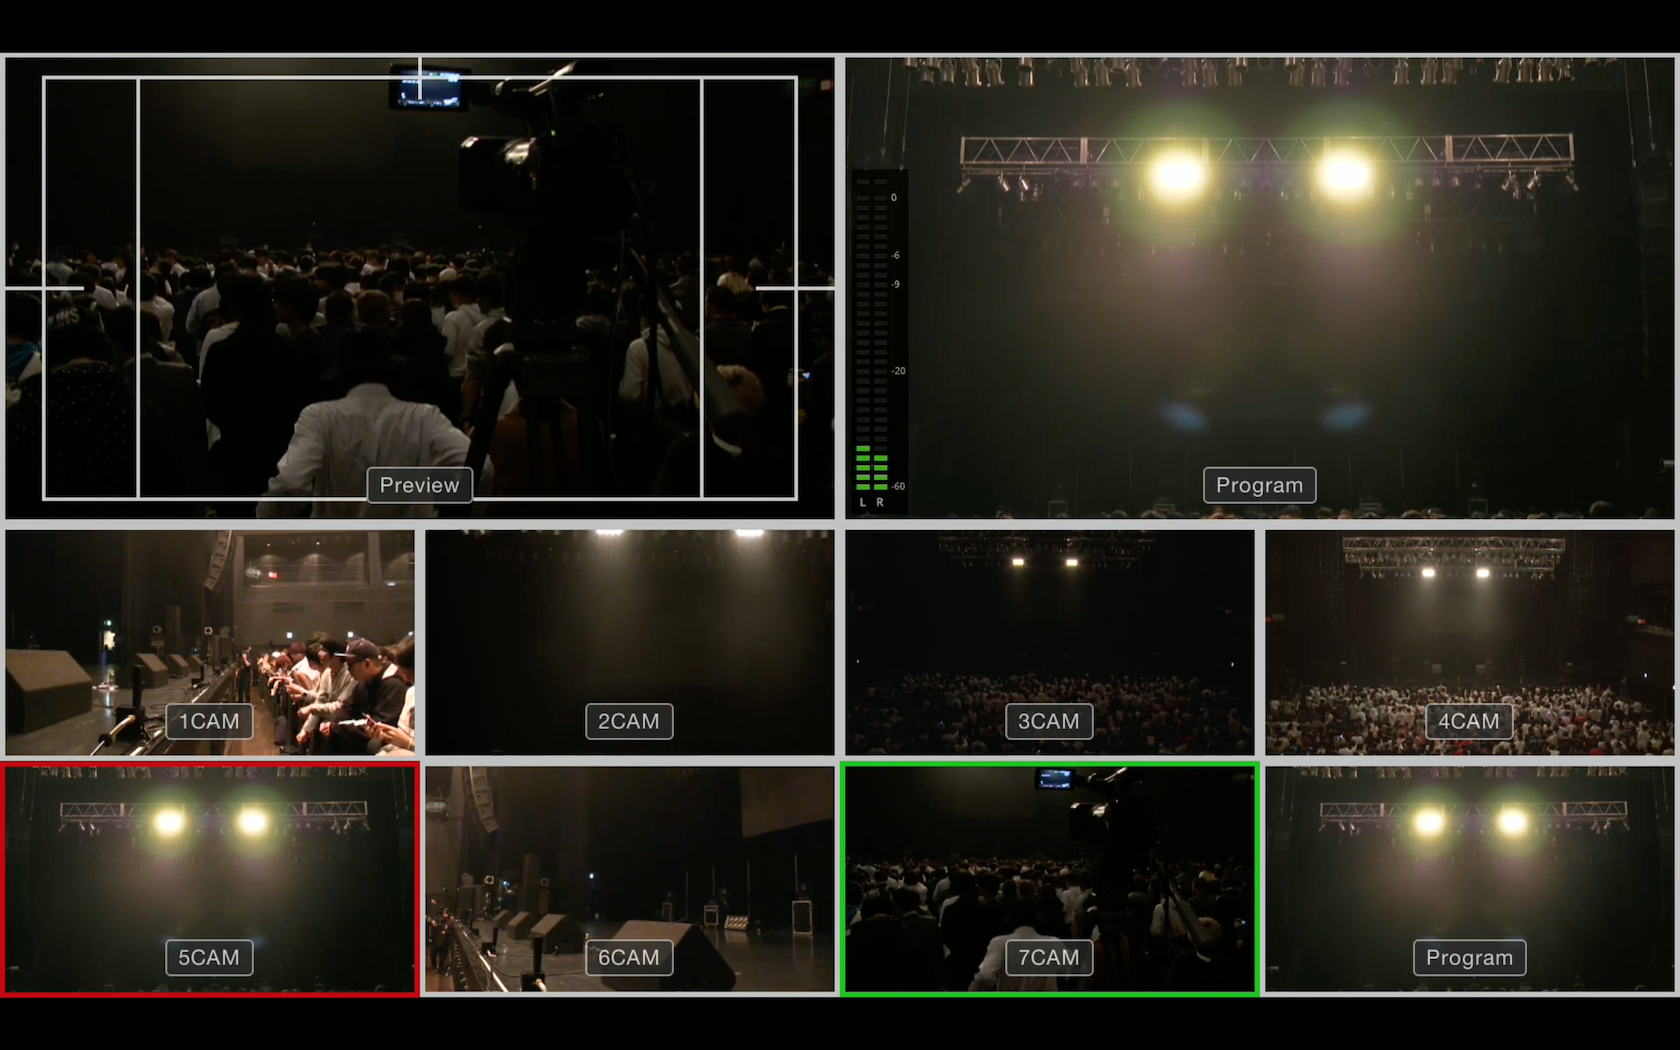
\includegraphics[bb=0 0 1680 1050,width=8cm]{img/mv-delay-actual.png}
%     \end{center}
%     \caption{TED HDMI 2.0 FMCカード (TB-FMCH-HDMI4K)}
%     \label{fig:ted-4k-fmc-card}
%   \end{minipage}
%   \begin{minipage}{0.5\hsize}
%     \begin{center}
%         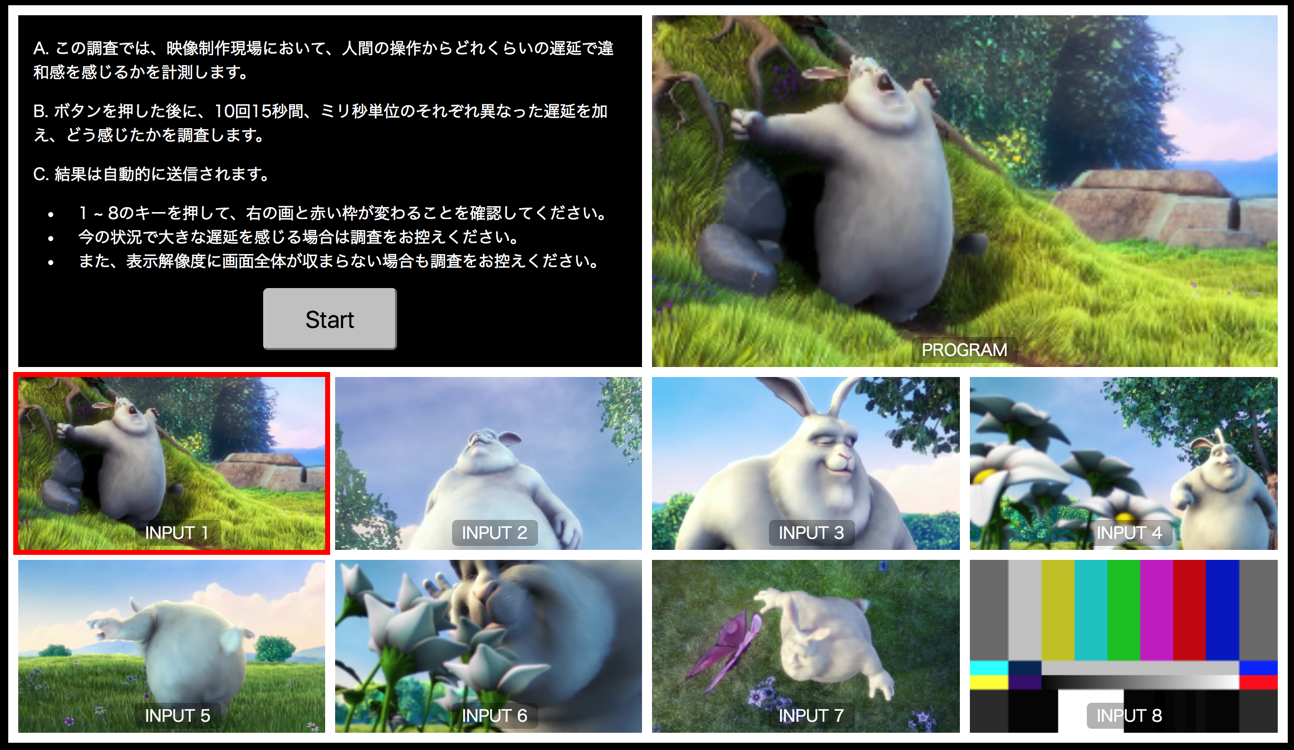
\includegraphics[bb=0 0 1294 750,width=8cm]{img/mv-delay-virtual.png}
%     \end{center}
%     \caption{TED HDMI 2.0 FMCカード (TB-FMCH-HDMI4K)}
%     \label{fig:ted-4k-fmc-card}
%   \end{minipage}
% \end{figure}

\begin{figure}[htbp]
  \begin{center}
    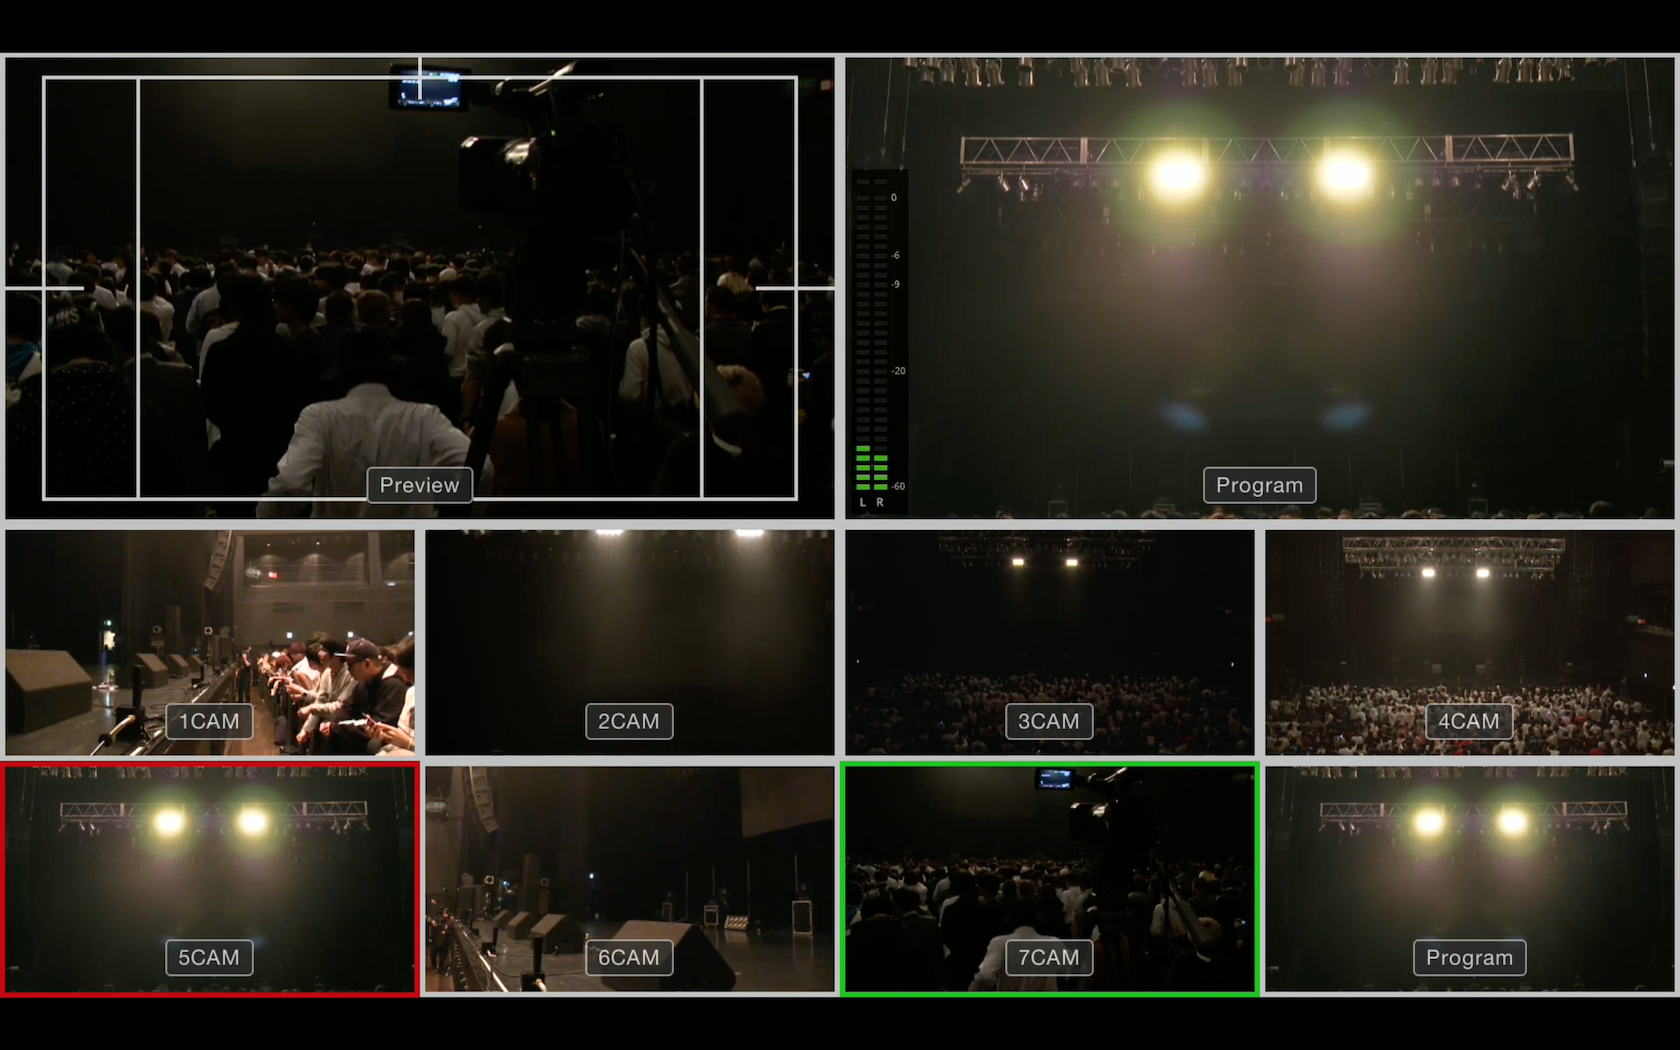
\includegraphics[bb=0 0 1680 1050,width=8cm]{img/mv-delay-actual.png}
  \end{center}
  \caption{}
  \label{fig:ted-4k-fmc-card}
\end{figure}
\begin{figure}[htbp]
  \begin{center}
    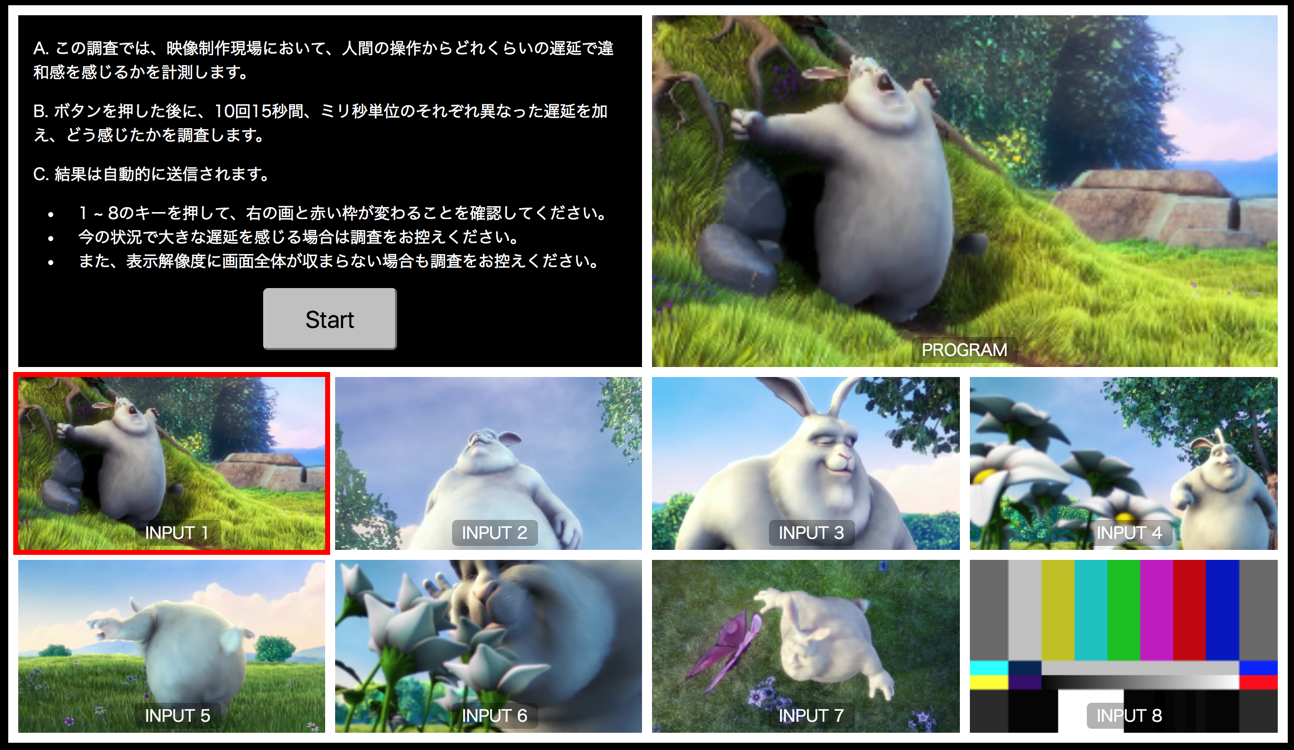
\includegraphics[bb=0 0 1294 750,width=8cm]{img/mv-delay-virtual.png}
  \end{center}
  \caption{今回の実験で使用したWebページ}
  \label{fig:ted-4k-fmc-card}
\end{figure}

\section{目的}

映像の制作の現場では、符号化・複合などによる映像の遅延を抑えることや、画質をそのまま伝送することがしばしば求められます。
このような背景から、4K映像を非圧縮のままIP伝送する技術の実証実験と、現場においてIP伝送を利用する際に問題となる点を洗い出します。?

% \section{構成}
